\section{Anhang}
\label{sec:Anhang}
\subsection{Restliche Tabellen und Plots zur Bestimmung der Grenzspannung}
\label{sec:Tabellen Rest}
\begin{table}[H]
    \centering
    \caption{Messwerte für die gelbe Spektrallinie.}
    \label{tab:gelb}
    \begin{tabular}{S[table-format=1.2] S[table-format=1.1]}
        \toprule
        $U_{\symup{B}} / \unit{\volt}$ & $I / \unit{\nano\ampere}$ \\
        \midrule
        0.20 &	0.94 \\
        0.25 &	0.56 \\
        0.30 &	0.30 \\
        0.35 &	0.16 \\
        0.40 &	0.08 \\
        0.45 &	0.02 \\
        0.5	 &  0    \\
        \bottomrule
    \end{tabular}
\end{table}

\begin{figure} [H]
    \centering
    \includegraphics{build/plot_gelb.pdf}
    \caption{Plot der Bremsspannung $U_{\symup{B}}$ gegen die Wurzel des Photostroms $I$ für die gelbe Spektrallinie.}
    \label{fig:plot_gelb}
\end{figure}

\begin{table}[H]
    \centering
    \caption{Messwerte für die grüne Spektrallinie.}
    \label{tab:gruen}
    \begin{tabular}{S[table-format=1.1] S[table-format=1.1]}
        \toprule
        $U_{\symup{B}} / \unit{\volt}$ & $I / \unit{\nano\ampere}$ \\
        \midrule
        0.1 &	8.6 \\
        0.2 &	4.7 \\
        0.3 &	1.9 \\
        0.4 &	0.6 \\
        0.5 &	0.2 \\
        0.6 &	0.0 \\
        \bottomrule
    \end{tabular}
\end{table}
  
\begin{figure} [H]
  \centering
  \includegraphics{build/plot_gruen.pdf}
  \caption{Plot der Bremsspannung $U_{\symup{B}}$ gegen die Wurzel des Photostroms $I$ für die grüne Spektrallinie.}
  \label{fig:plot_gruen}
\end{figure}

\begin{table}[H]
    \centering
    \caption{Messwerte für die erste violette Spektrallinie.}
    \label{tab:violett1}
    \begin{tabular}{S[table-format=1.1] S[table-format=2.2]}
        \toprule
        $U_{\symup{B}} / \unit{\volt}$ & $I / \unit{\nano\ampere}$ \\
        \midrule
        0.0 &	29.0 \\
        0.1 &	24.0 \\
        0.2 &	20.0 \\
        0.3 &	16.0 \\
        0.4 &	12.0 \\
        0.5 &	8.8  \\
        0.6 &	5.8  \\
        0.7 &	3.5  \\
        0.8 &	2.0  \\
        0.9 &	1.0  \\
        1.0 &	0.4  \\
        1.1 &	0.05 \\
        1.2 &	0.00 \\
    \end{tabular}
\end{table}

\begin{figure} [H]
  \centering
  \includegraphics{build/plot_violett_1.pdf}
  \caption{Plot der Bremsspannung $U_{\symup{B}}$ gegen die Wurzel des Photostroms $I$ für die erste violette Spektrallinie.}
  \label{fig:plot_violett_1}
\end{figure}

\begin{table}[H]
    \centering
    \caption{Messwerte für die zweite violette Spektrallinie.}
    \label{tab:violett2}
    \begin{tabular}{S[table-format=1.1] S[table-format=2.2]}
        \toprule
        $U_{\symup{B}} / \unit{\volt}$ & $I / \unit{\nano\ampere}$ \\
        \midrule
        0.0 &	11.0 \\
        0.1 &	10.0 \\
        0.2 &	9.6  \\
        0.3 &	7.8  \\
        0.4 &	6.4  \\
        0.5 &	5.0  \\
        0.6 &	3.6  \\
        0.7 &	2.6  \\
        0.8 &	1.7  \\
        0.9 &	1.0  \\
        1.0 &	0.6  \\
        1.1 &	0.25 \\
        1.2 &	0.10 \\
        1.3 &	0.00 \\
    \end{tabular}
\end{table}

\begin{figure} [H]
  \centering
  \includegraphics{build/plot_violett_2.pdf}
  \caption{Plot der Bremsspannung $U_{\symup{B}}$ gegen die Wurzel des Photostroms $I$ für die zweite violette Spektrallinie.}
  \label{fig:plot_violett_2}
\end{figure}

\subsection{Originaldaten}
\centering
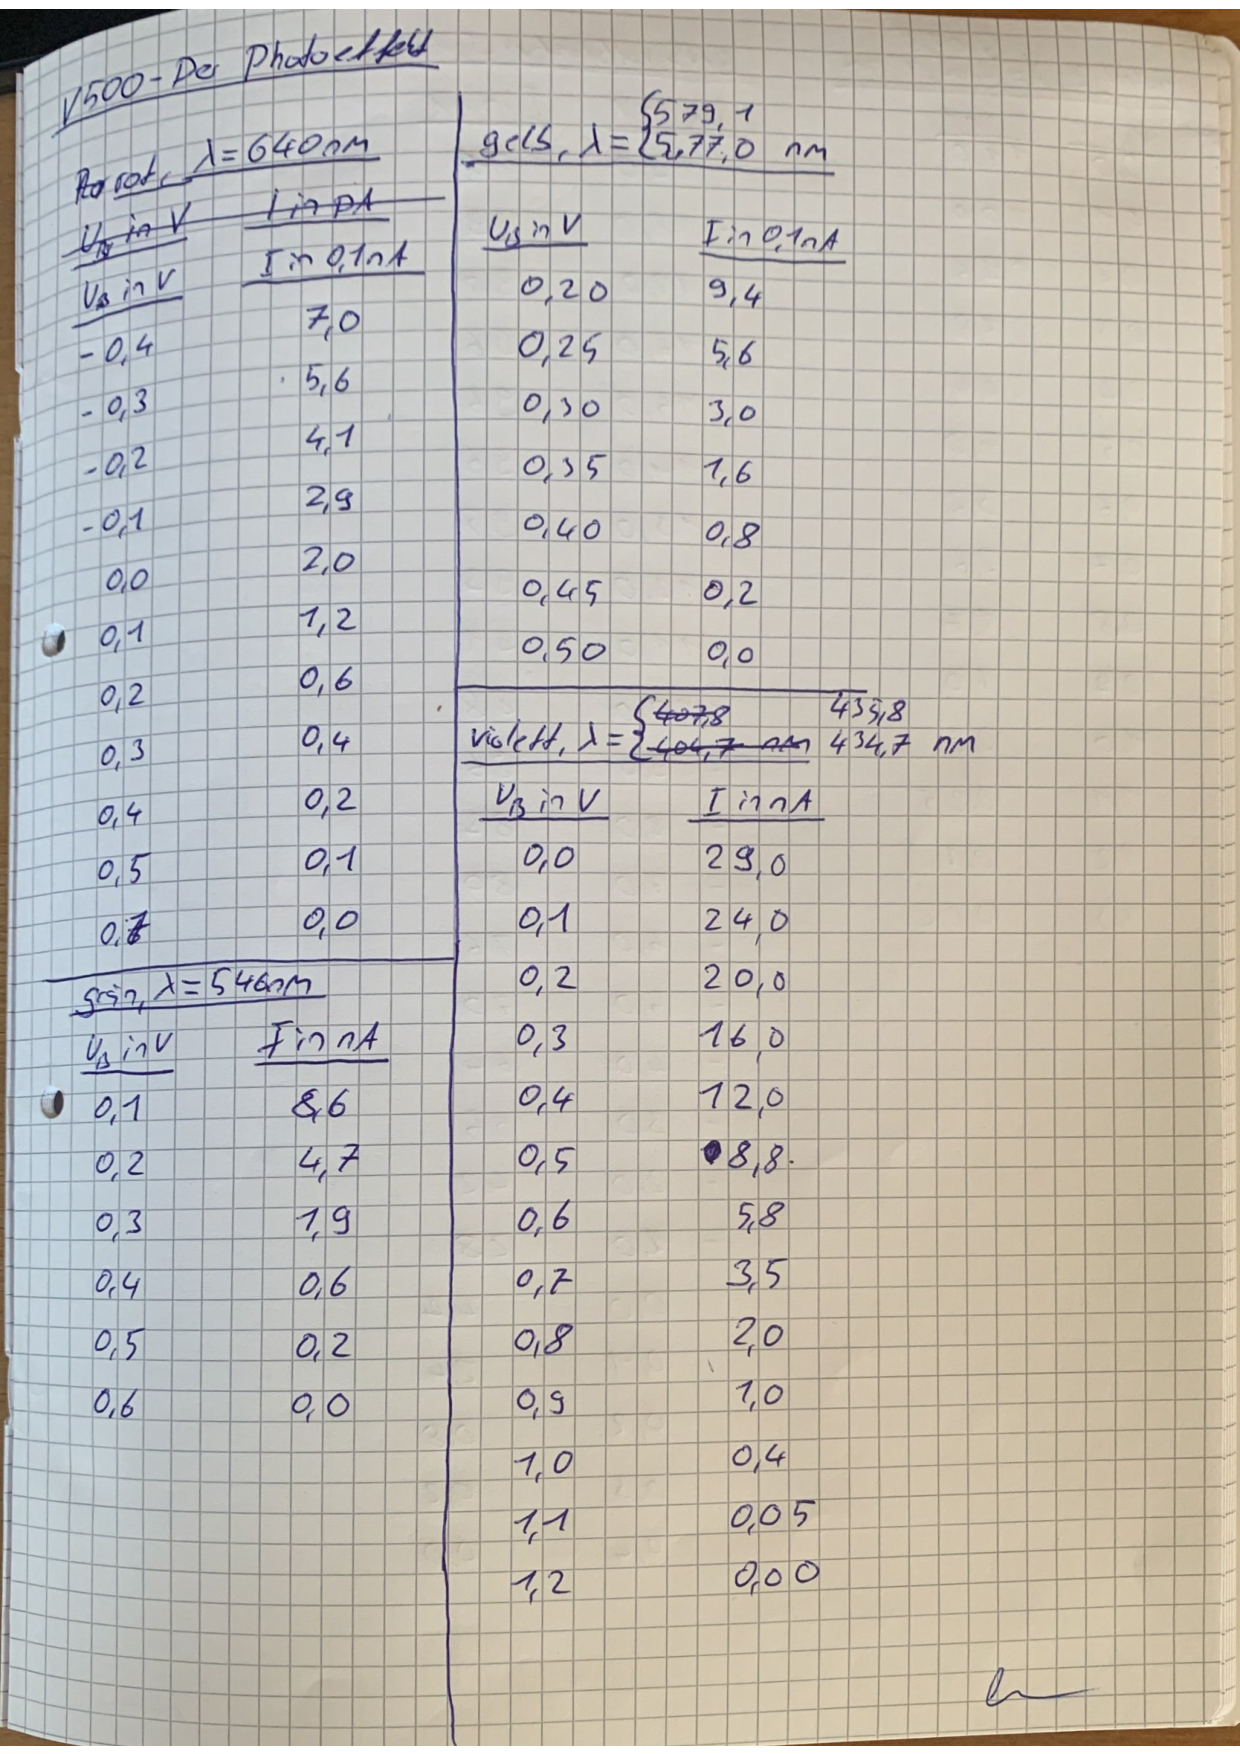
\includegraphics[height=18cm]{content/pics/originaldaten/Originaldaten_1.pdf}
\newpage
\centering
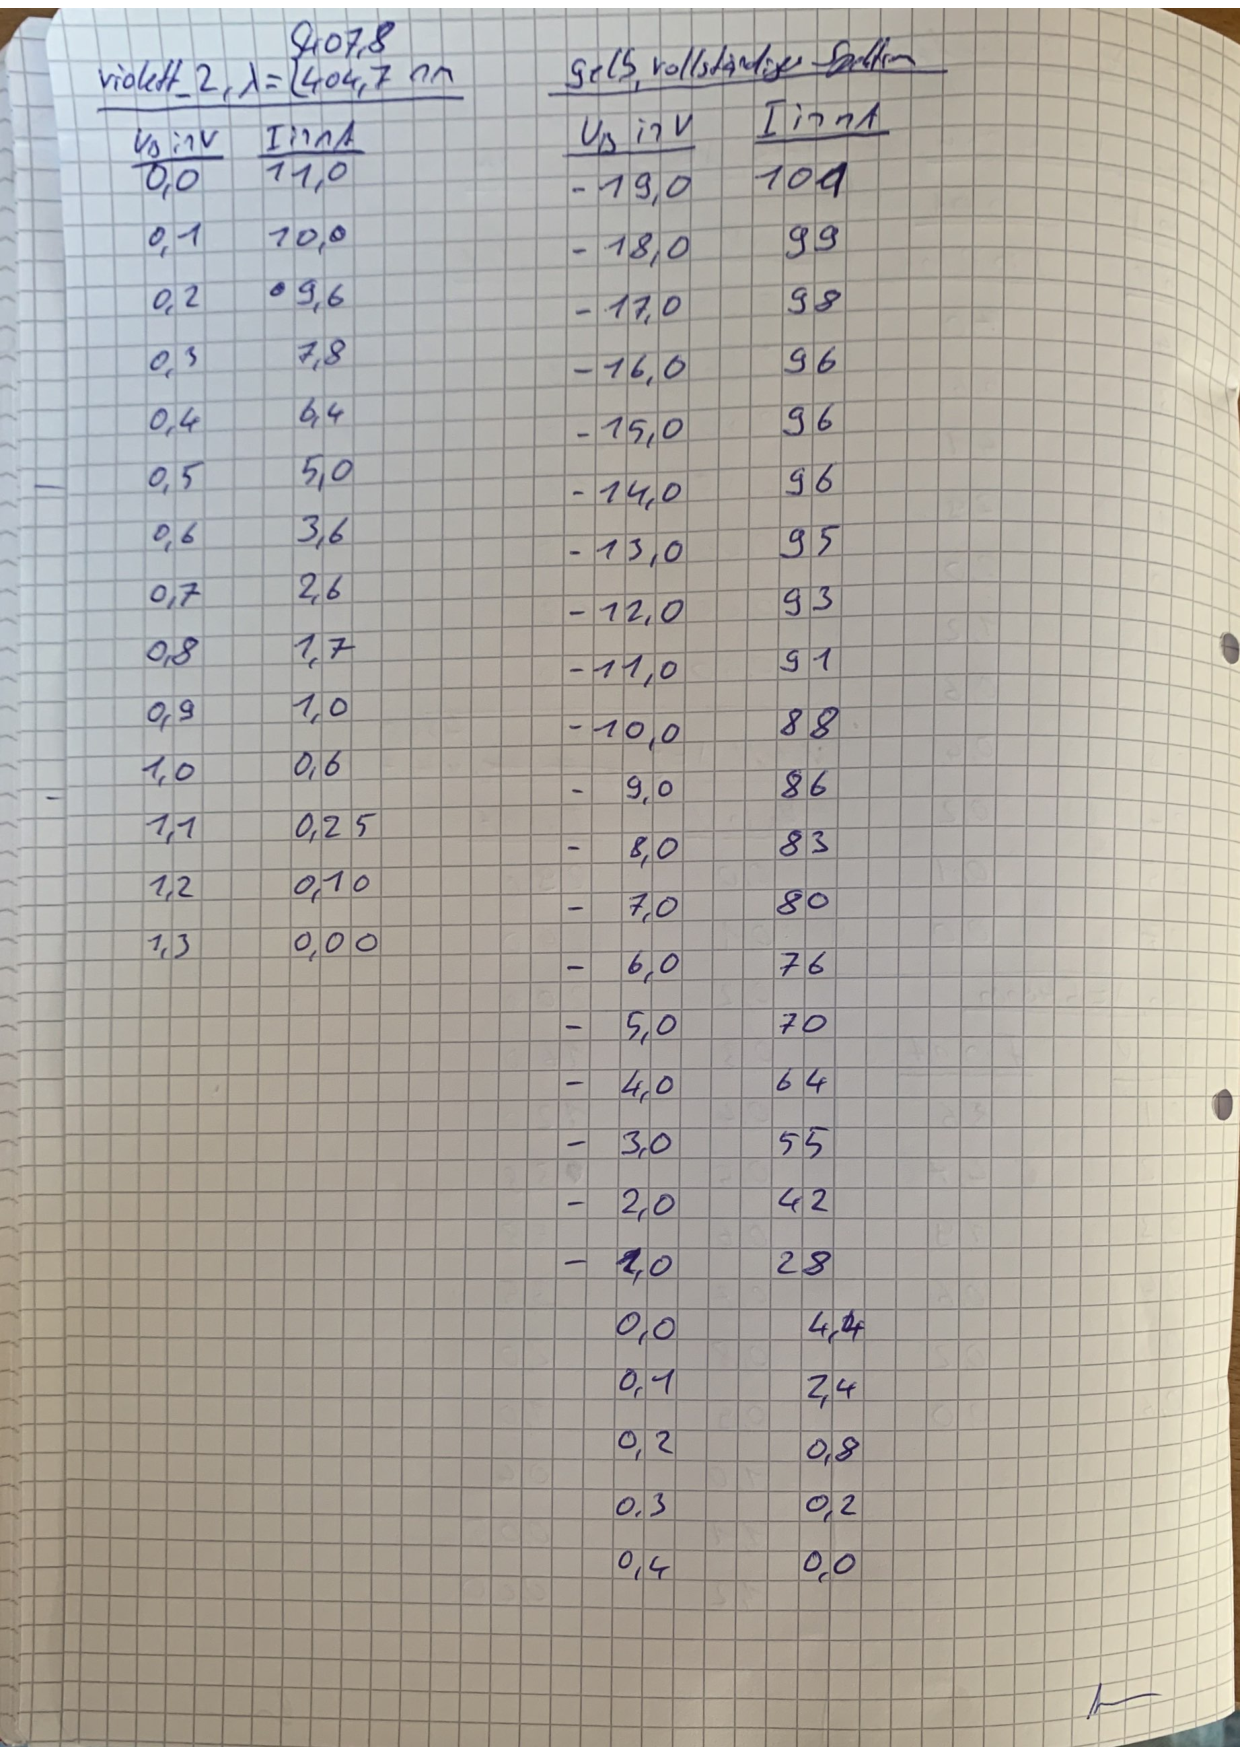
\includegraphics[height=18cm]{content/pics/originaldaten/Originaldaten_2.pdf}